\documentclass[a4paper,12pt]{article}
\usepackage[utf8]{inputenc}
\usepackage[francais]{babel}
\usepackage[T1]{fontenc}
\usepackage{graphicx}
\usepackage{listingsutf8}
\usepackage[colorlinks,urlcolor=blue]{hyperref} %hyperlinks
% \usepackage[nottoc,notlot,notlof]{tocbibind} %To bind the table of contents to the bibligoraphy
% \usepackage[page,toc,titletoc,title]{appendix} %To add appendices to the document
\usepackage{../../packages/tikz-uml} %UML elements

\title{
  HMIN122M Rendu \\
  \large TP2
}
\author{Bachar Rima \and Joseph Saba \and Tasnim Muhammad}
\date{27 septembre 2018}

\lstset{
  language=SQL,
  basicstyle=\ttfamily\small,
  keywordstyle=\color{blue!60},
  commentstyle=\color{red!80}\upshape,
  stringstyle=\color{purple},
  showstringspaces=false,
  rulecolor=\color{black!30},
  numberstyle=\footnotesize,
  numbers=left,
  breaklines=true,
  breakatwhitespace=true,
  tabsize=3,
  frame=single,
  framextopmargin=2pt,
  framexbottommargin=2pt,
  backgroundcolor=\color{gray!10},
  captionpos=b,
  inputencoding=utf8,
  extendedchars=true,
  literate={á}{{\'a}}1 {é}{{\'e}}1 {í}{{\'i}}1 {ó}{{\'o}}1 {ú}{{\'u}}1 {Á}{{\'A}}1 {É}{{\'E}}1 {Í}{{\'I}}1 {Ó}{{\'O}}1 {Ú}{{\'U}}1 {à}{{\`a}}1 {è}{{\`e}}1 {ì}{{\`i}}1 {ò}{{\`o}}1 {ù}{{\`u}}1 {À}{{\`A}}1 {È}{{\'E}}1 {Ì}{{\`I}}1 {Ò}{{\`O}}1 {Ù}{{\`U}}1 {ä}{{\"a}}1 {ë}{{\"e}}1 {ï}{{\"i}}1 {ö}{{\"o}}1 {ü}{{\"u}}1 {Ä}{{\"A}}1 {Ë}{{\"E}}1 {Ï}{{\"I}}1 {Ö}{{\"O}}1 {Ü}{{\"U}}1 {â}{{\^a}}1 {ê}{{\^e}}1 {î}{{\^i}}1 {ô}{{\^o}}1 {û}{{\^u}}1 {Â}{{\^A}}1 {Ê}{{\^E}}1 {Î}{{\^I}}1 {Ô}{{\^O}}1 {Û}{{\^U}}1 {œ}{{\oe}}1 {Œ}{{\OE}}1 {æ}{{\ae}}1 {Æ}{{\AE}}1 {ß}{{\ss}}1 {ű}{{\H{u}}}1 {Ű}{{\H{U}}}1 {ő}{{\H{o}}}1 {Ő}{{\H{O}}}1 {ç}{{\c c}}1 {Ç}{{\c C}}1 {ø}{{\o}}1 {å}{{\r a}}1 {Å}{{\r A}}1 {€}{{\euro}}1 {£}{{\pounds}}1 {«}{{\guillemotleft}}1 {»}{{\guillemotright}}1 {ñ}{{\~n}}1 {Ñ}{{\~N}}1 {¿}{{?`}}1
}

\begin{document}
\pagestyle{plain}

\maketitle

{
  \hypersetup{linkcolor=black}
  \tableofcontents
}

\section{Sélection}
\subsection{Question 1}
\begin{description}
  \item [@script\_table.sql :] création des tables de la base de données.
  \item [@script\_remplissage.sql :] remplissage des tables créées.
  \item [set autotrace on :] faire des statistiques sur les requêtes exécutées.
  \item [set linesize 200 :] étendre la taille des tables affichées pour une meilleure visibilité.
\end{description}

\subsection{Question 2}
\begin{lstlisting}[caption={requêtes permettant d'expliquer le plan d'exécution affichant le nom des villes dont le numéro insee est 34172}, label={lst:question_2}]
  explain plan for select nom from ville where insee='34172';
  select plan_table_output from table(dbms_xplan.display());
\end{lstlisting}

\begin{figure}[!ht]
  \centering
  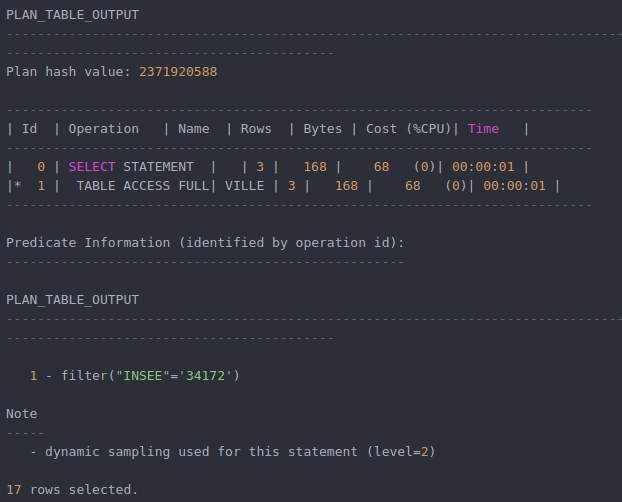
\includegraphics[scale=0.6]{images/q2_1.png}
  \caption{Plan d'exécution}
\end{figure}

\begin{figure}[!ht]
  \centering
  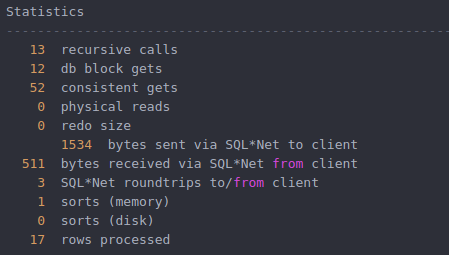
\includegraphics[scale=0.6]{images/q2_2.png}
  \caption{Statistiques}
\end{figure}

\newpage

\subsection{Question 3}
\begin{minipage}{\linewidth}
  \begin{lstlisting}[caption={ajout d'une clé primaire sur la table Ville en utilisant l'attribut insee}]
    alter table ville add constraint PK_VILLE primary key(insee);
  \end{lstlisting}
\end{minipage}

\subsection{Question 4}
Avant l'ajout d'une clé primaire à la table \texttt{Ville}, l'algorithme choisi par l'optimiseur pour la requête est \textit{Table Access Full}. Ce dernier est généralement gourmand en termes de consommation de ressources, vu qu'il doit balayer la table entièrement, ligne par ligne, et attribut par attribut.

Après l'ajout d'une clé primaire à la table \texttt{Ville}, notamment sur l'attribut \textbf{insee}, l'algorithme choisi par l'optimiseur sera \textit{Index Unique Scan}. Ce dernier permet de parcourir la table selon l'index placé sur la clé primaire et est ainsi moins gourmand en termes de consommation de ressources.

\section{Jointure}
\subsection{Question 5}
\begin{lstlisting}[caption={requêtes permettant d'expliquer le plan d'exécution affichant le nom du département pour la ville dont le numéro insee est 34172}, label={lst:question_5}]
  explain plan for select departement.nom from departement, ville where insee='34172' and departement.id = ville.dep;
  select plan_table_output from table(dbms_xplan.display());
\end{lstlisting}

\begin{figure}[!ht]
  \centering
  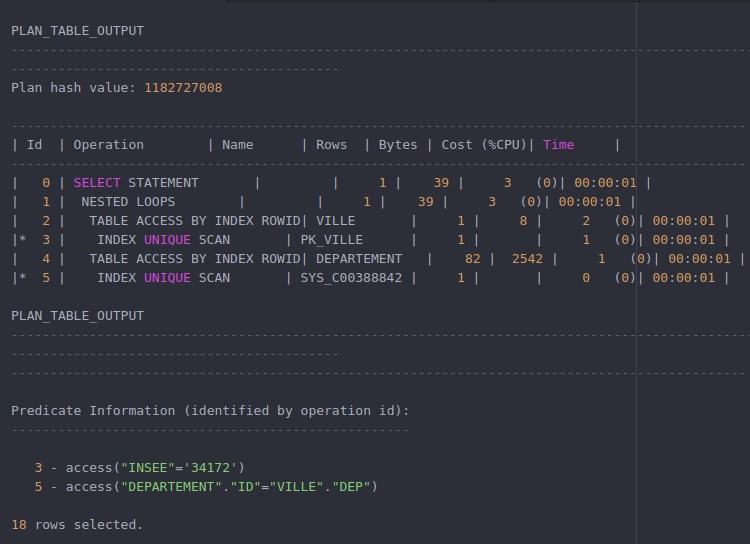
\includegraphics[scale=0.6]{images/q5_1.png}
  \caption{Plan d'exécution}
\end{figure}

\begin{figure}[!ht]
  \centering
  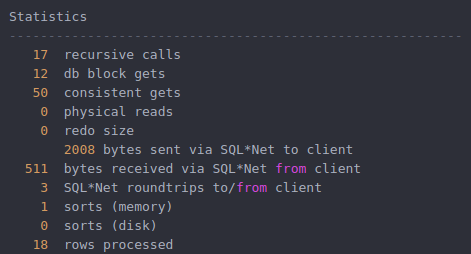
\includegraphics[scale=0.6]{images/q5_2.png}
  \caption{Statistiques}
\end{figure}

\newpage

\subsection{Question 6}
Dans la requête précédente, l'optimiseur a choisi les algorithmes \textit{Index Unique Scan} puis \textit{Nested Loops} lors de la jointure des tables \texttt{Ville} et \texttt{Departement}, vu que cette dernière se fait sur leurs attributs clés primaires, respectivement \textbf{insee} et \textbf{id}, après avoir sélectionné les tuples vérifiant une condition de sélection (notamment, la ville ayant le code \textbf{insee} $34172$).

D'autre part, la requête courante ne spécifie aucune condition de sélection précédant la jointure sur les deux tables. Par conséquent, l'optimiseur a choisi les algorithmes \textit{Table Access Full} pour balayer les tables et \textit{Hash Join} pour faire la jointure.

\begin{lstlisting}[caption={requêtes permettant d'expliquer le plan d'exécution affichant le nom du département pour toutes les villes}, label={lst:question_6}]
  explain plan for select departement.nom from departement, ville where departement.id = ville.dep;
  select plan_table_output from table(dbms_xplan.display());
\end{lstlisting}

\begin{figure}[!ht]
  \centering
  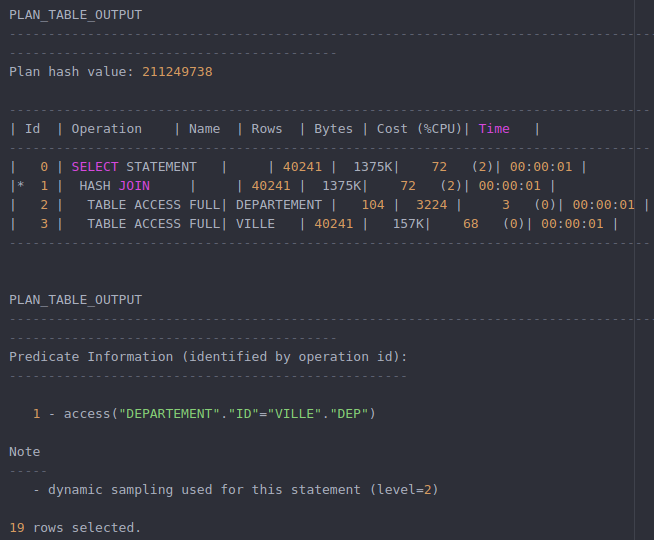
\includegraphics[scale=0.6]{images/q6_1.png}
  \caption{Plan d'exécution}
\end{figure}

\begin{figure}[!ht]
  \centering
  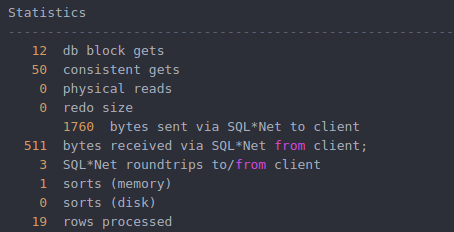
\includegraphics[scale=0.6]{images/q6_2.png}
  \caption{Statistiques}
\end{figure}

\newpage

\subsection{Question 7}
Pour la requête du listing \ref{lst:question_7.1}, l'optimiseur a choisi les algorithmes \textit{Index Unique Scan} pour sélectionner le département ayant un \textbf{id} (clé primaire de la table \texttt{Departement}) $91$ et \textit{Table Access Full} pour balayer la table \texttt{Ville}, vu que la jointure se fait sur un attribut non clé primaire de celle-ci. Suite à cette opération, l'algorithme \textit{Nested Loops} est utilisé lors de l'opération de jointure sur ces deux tables.

Pour la requête du listing \ref{lst:question_7.2}, par contre, en absence d'une opération de jointure, l'optimiseur choisit l'algorithme \textit{Index Unique Scan} sur l'attribut clé primaire \textbf{id} de la table \texttt{Departement} pour la valeur $92$.

\begin{lstlisting}[caption={requêtes permettant d'expliquer le plan d'exécution affichant le nom des villes et du département dont le numéro est 91 (id)}, label={lst:question_7.1}]
  explain plan for select ville.nom, departement.nom from ville, departement where departement.id='91' and ville.dep=departement.id;
  select plan_table_output from table(dbms_xplan.display());
\end{lstlisting}

\begin{figure}[!ht]
  \centering
  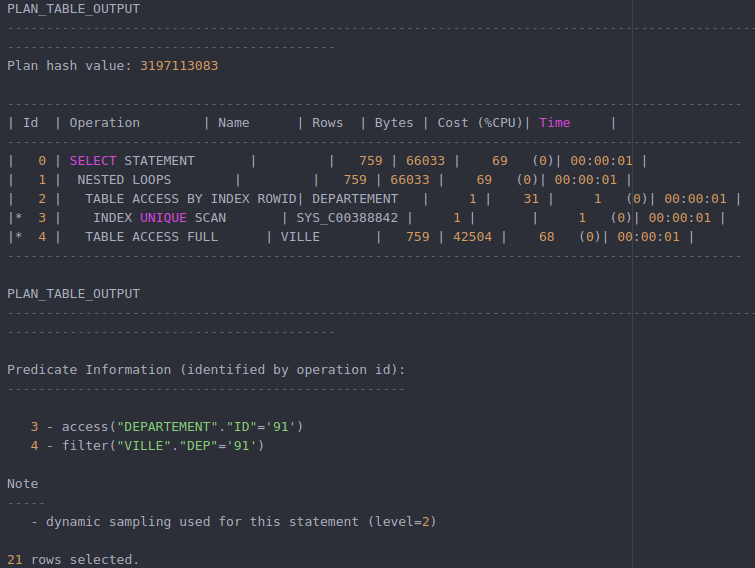
\includegraphics[scale=0.6]{images/q7_1.png}
  \caption{Plan d'exécution}
\end{figure}

\begin{figure}[!ht]
  \centering
  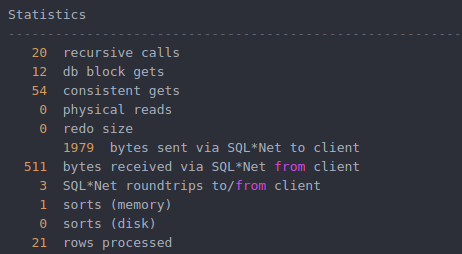
\includegraphics[scale=0.6]{images/q7_2.png}
  \caption{Statistiques}
\end{figure}

\begin{lstlisting}[caption={requêtes permettant d'expliquer le plan d'exécution affichant le nom du département dont le numéro est 92}, label={lst:question_7.2}]
  explain plan for select departement.nom from departement where departement.id='92';
  select plan_table_output from table(dbms_xplan.display());
\end{lstlisting}

\begin{figure}[!ht]
  \centering
  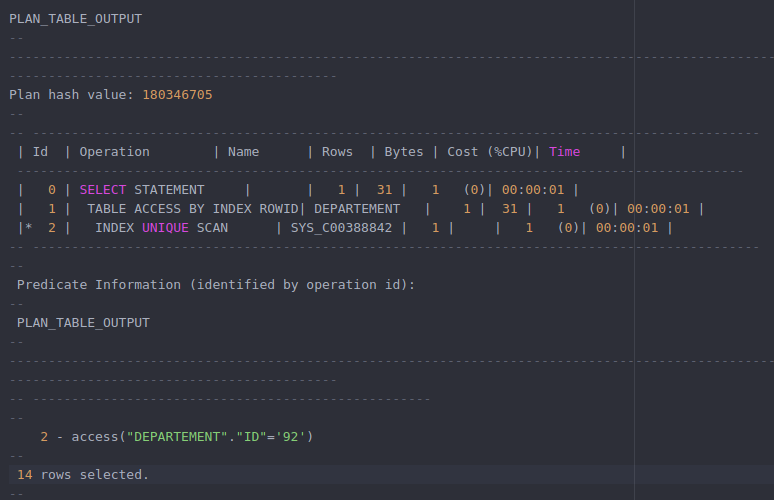
\includegraphics[scale=0.6]{images/q7_3.png}
  \caption{Plan d'exécution}
\end{figure}

\begin{figure}[!ht]
  \centering
  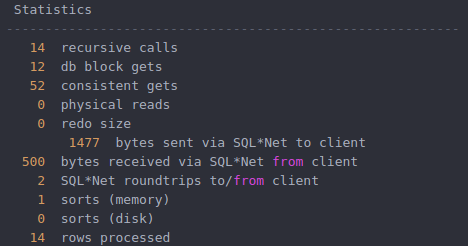
\includegraphics[scale=0.6]{images/q7_4.png}
  \caption{Statistiques}
\end{figure}

\newpage

\section{Modification du comportement de l'optimiseur}
\subsection{Question 8}
En choissisant explicitement l'algorithme \textit{Nested Loops} pour les requêtes des listings \ref{lst:question_5} et \ref{lst:question_7.1}, on obtient les mêmes résultats.

D'autre part, quand on force l'optimiseur à utiliser l'algorithme \textit{Nested Loops} pour la requête du listing \ref{lst:question_6} (cf. listing \ref{lst:question_8}), le nombre d'appels récursifs\footnote{\textit{recursive calls}} augmente considérablement (cf. Figure \ref{fig:q8_2}) par rapport à l'algorithme \textit{Hash Join} utilisé par défaut par l'optimiseur pour cette requête.

\begin{lstlisting}[caption={requêtes permettant d'expliquer le plan d'exécution affichant le nom du département pour toutes les villes, en forçant l'utilisation de l'algorithme de jointure Nested Loops}, label={lst:question_8}]
  explain plan for select /*+ use_nl(departement ville)*/ departement.nom from departement, ville where departement.id = ville.dep;
  select plan_table_output from table(dbms_xplan.display());
\end{lstlisting}

\begin{figure}[!ht]
  \centering
  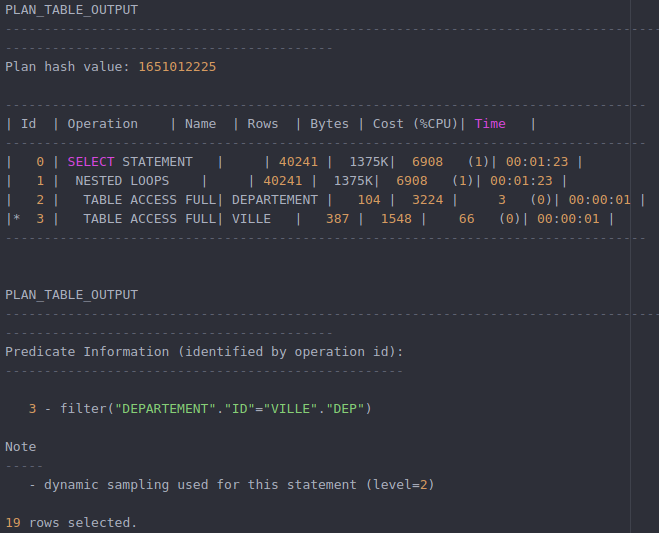
\includegraphics[scale=0.6]{images/q8_1.png}
  \caption{Plan d'exécution}
\end{figure}

\begin{figure}[!ht]
  \centering
  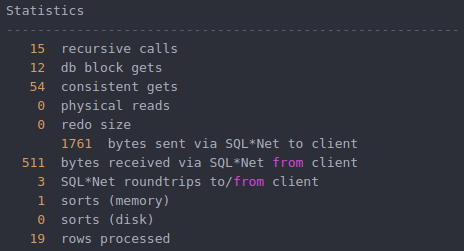
\includegraphics[scale=0.6]{images/q8_2.png}
  \caption{Statistiques}
  \label{fig:q8_2}
\end{figure}

\newpage

\section{Utilisation d'index}
\subsection{Question 9}
\begin{lstlisting}[caption={ajout d'un index secondaire sur l'attribut dep de la table Ville}]
  create index idx_dep_ville on ville(dep);
\end{lstlisting}

L'ajout d'un index secondaire sur l'attribut \textbf{dep} de la table \texttt{Ville} n'affecte pas les plans d'exécution des requêtes des listings  \ref{lst:question_2} et \ref{lst:question_5}, vu que cet attribut ne figure pas dans ces requêtes.

D'autre part, cet ajout change le plan d'exécution de la requête du listing \ref{lst:question_6}, vu que celle-ci contient bien cet attribut. En effet, l'ajout d'un index sur cet attribut permet à l'optimiseur de choisir l'algorithme \textit{Index Fast Full Scan} (cf. Figure \ref{fig:qu9_1}) pour balayer la table selon cet index, au lieu d'utiliser \textit{Table Full Scan} choisi précédemment.

En outre, cet ajout change le plan d'exécution de la requête du listing \ref{lst:question_7.1}, vu que celle-ci contient bien cet attribut. En effet, l'ajout d'un index sur cet attribut permet à l'optimiseur de choisir l'algorithme \textit{Index Range Scan} (cf. Figure \ref{fig:qu9_3}) pour balayer la table selon cet index, au lieu d'utiliser \textit{Table Full Scan} choisi précédemment.

\begin{figure}[!ht]
  \centering
  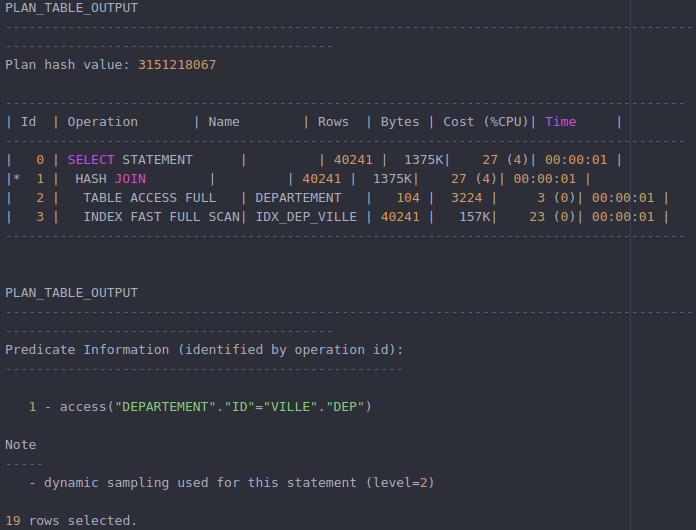
\includegraphics[scale=0.6]{images/q9_1.png}
  \caption{Plan d'exécution}
  \label{fig:qu9_1}
\end{figure}

\begin{figure}[!ht]
  \centering
  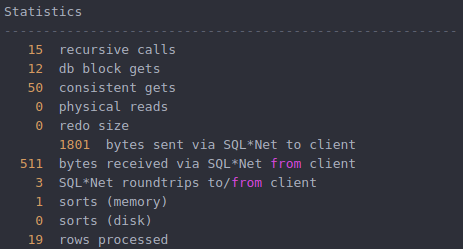
\includegraphics[scale=0.6]{images/q9_2.png}
  \caption{Statistiques}
\end{figure}

\newpage

\begin{figure}[!ht]
  \centering
  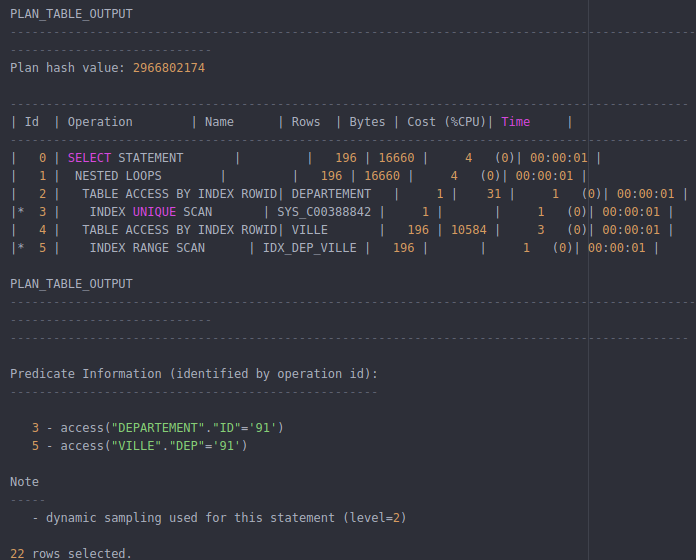
\includegraphics[scale=0.6]{images/q9_3.png}
  \caption{Plan d'exécution}
  \label{fig:qu9_3}
\end{figure}

\begin{figure}[!ht]
  \centering
  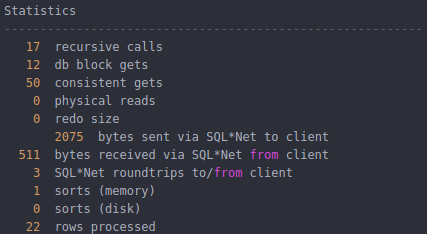
\includegraphics[scale=0.6]{images/q9_4.png}
  \caption{Statistiques}
\end{figure}

\newpage

\subsection{Question 10}
\begin{minipage}{\linewidth}
  \begin{lstlisting}[caption={requêtes permettant d'expliquer le plan d'exécution affichant le nom des villes, de leurs départements et de leurs régions}, label={lst:question_10}]
    explain plan for select ville.nom, departement.nom, region.nom from ville, departement, region where ville.dep = departement.id and departement.reg = region.id;
    select plan_table_output from table(dbms_xplan.display());
  \end{lstlisting}
\end{minipage}

\begin{figure}[!ht]
  \centering
  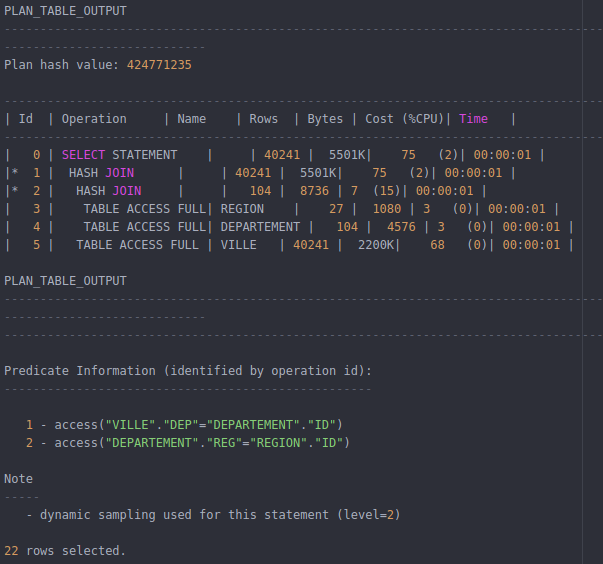
\includegraphics[scale=0.6]{images/q10_1.png}
  \caption{Plan d'exécution}
\end{figure}

\begin{figure}[!ht]
  \centering
  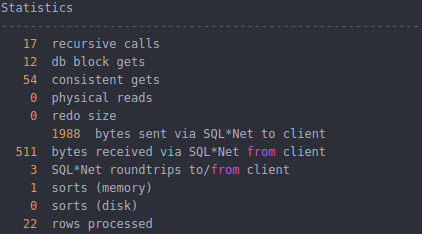
\includegraphics[scale=0.6]{images/q10_2.png}
  \caption{Statistiques}
\end{figure}

\newpage

\subsection{Question 11}
\begin{lstlisting}[caption={ajout d'un index secondaire sur l'attribut reg de la table Departement}]
  create index idx_reg_departement on departement(reg);
\end{lstlisting}

La ré-exécution de la requête du listing \ref{lst:question_10}, suite à l'ajout de l'index secondaire sur l'attribut \textbf{reg} de la table \texttt{Departement}, fournit les résultats affichés dans les figures \ref{fig:11_1} et \ref{fig:11_2}.

\begin{figure}[!ht]
  \centering
  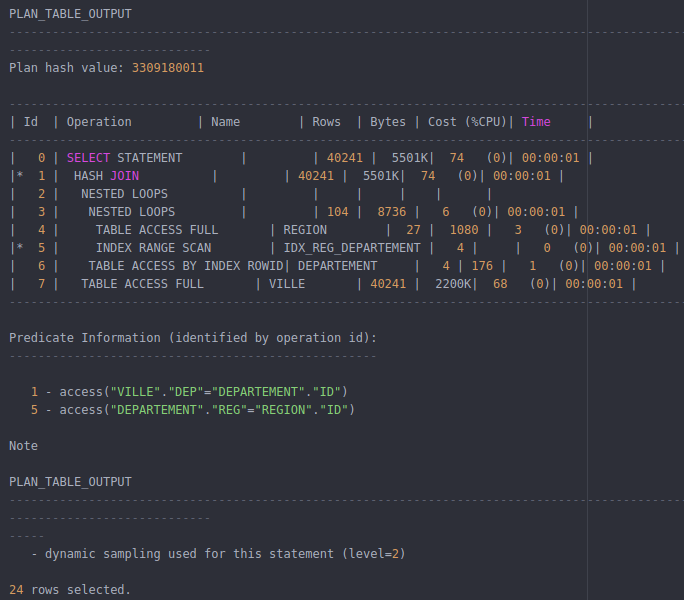
\includegraphics[scale=0.6]{images/q11_1.png}
  \caption{Plan d'exécution}
  \label{fig:11_1}
\end{figure}

\begin{figure}[!ht]
  \centering
  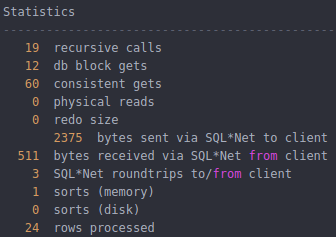
\includegraphics[scale=0.6]{images/q11_2.png}
  \caption{Statistiques}
  \label{fig:11_2}
\end{figure}

\newpage

\subsection{Question 12}
\begin{lstlisting}[caption={requêtes permettant d'expliquer le plan d'exécution affichant le nom des villes, de leurs départements et de la région pour la région dont le numéro (id) est 91}]
  explain plan for select ville.nom, departement.nom, region.nom from ville, departement, region where region.id=91 and ville.dep=departement.id and departement.reg=region.id;
  select plan_table_output from table(dbms_xplan.display());
\end{lstlisting}

\begin{figure}[!ht]
  \centering
  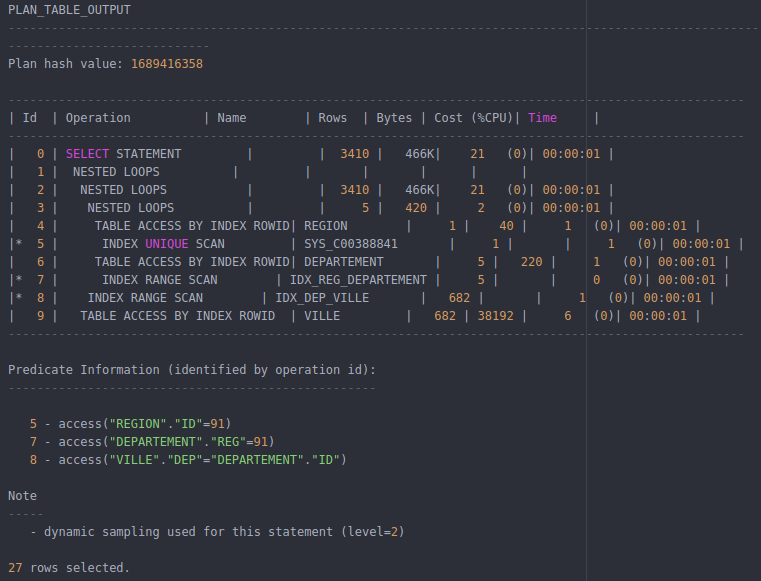
\includegraphics[scale=0.6]{images/q12_1.png}
  \caption{Plan d'exécution}
\end{figure}

\begin{figure}[!ht]
  \centering
  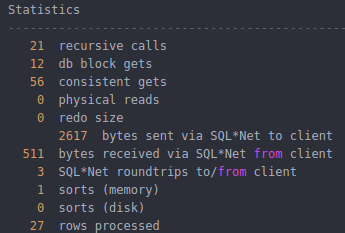
\includegraphics[scale=0.6]{images/q12_2.png}
  \caption{Statistiques}
\end{figure}

\newpage

\subsection{Question 13}
L'ajout d'un index secondaire sur l'attribut \textbf{dep} de la table \texttt{Ville} permet à l'optimiseur de choisir l'algorithme \textit{Index Range Scan} pour balayer cette table selon cet index, et permet par conséquent d'optimiser les accès aux tuples et moins de consommation en termes de temps d'exécution et de mémoire.

\begin{lstlisting}[caption={requêtes permettant d'expliquer le plan d'exécution affichant le nom des villes dont le numéro de département (dep) commence par 7}]
  explain plan for select ville.nom from ville where ville.dep LIKE '7%';
  select plan_table_output from table(dbms_xplan.display());
\end{lstlisting}

\begin{figure}[!ht]
  \centering
  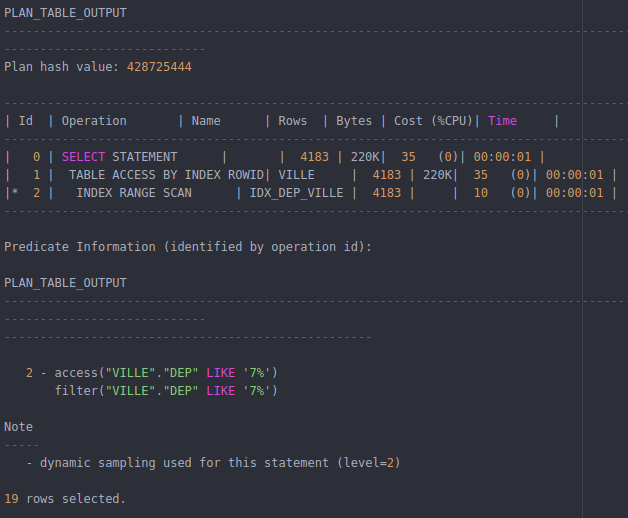
\includegraphics[scale=0.6]{images/q13_1.png}
  \caption{Plan d'exécution}
\end{figure}

\begin{figure}[!ht]
  \centering
  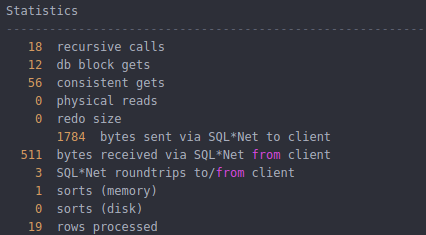
\includegraphics[scale=0.6]{images/q13_2.png}
  \caption{Statistiques}
\end{figure}

\newpage

\section{Les statistiques des tables}
\subsection{Question 14}
\begin{lstlisting}[caption={requêtes permettant de recalculer les statistiques sur les tables Ville, Departement et Region afin de visualiser les coûts des différents plans d'exécution qui y sont associés}]
  exec dbms_stats.gather_table_stats('brima','ville'); --adds the cost details for table 'ville'
  exec dbms_stats.gather_table_stats('brima','departement'); --adds the cost details for table 'departement'
  exec dbms_stats.gather_table_stats('brima','region'); --adds the cost details for table 'region'
  SELECT * FROM USER_TAB_COL_STATISTICS; --visualize the obtained tables describing these costs
\end{lstlisting}

\begin{figure}[!ht]
  \centering
  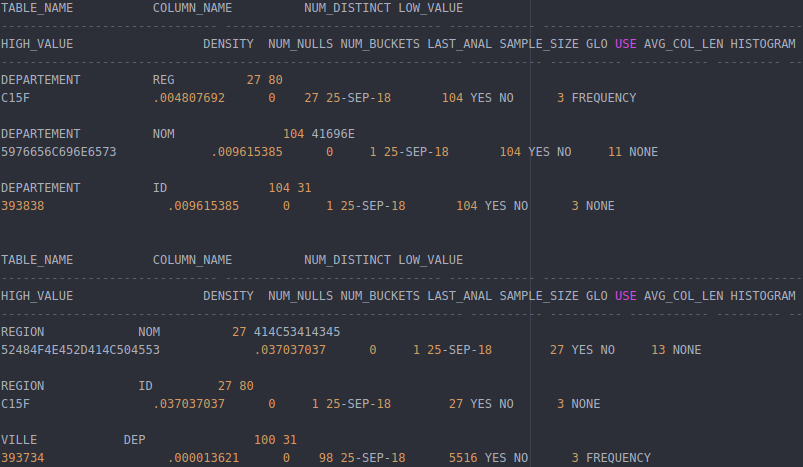
\includegraphics[scale=0.55]{images/q14_1.png}
  \caption{Coûts des différents plans d'exécution des tables Departement et Region}
\end{figure}

\begin{figure}[!ht]
  \centering
  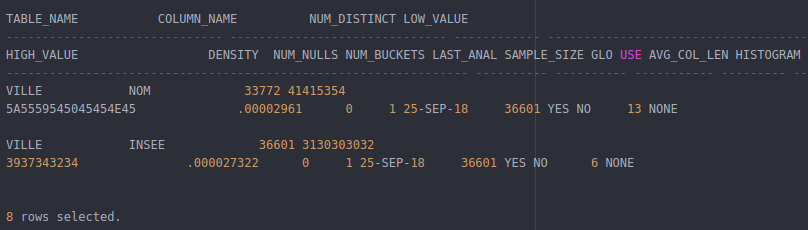
\includegraphics[scale=0.55]{images/q14_2.png}
  \caption{Coûts des différents plans d'exécution de la table Ville}
\end{figure}

\end{document}
